\lecture{5}{lun 01 mag 2023 17:12}{Stabilità}
	\lablsection{Stabilità}
        \twomini{
		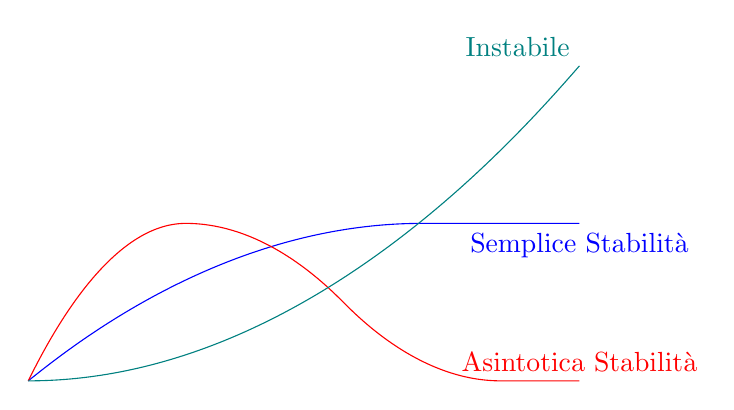
\begin{tikzpicture}
			\assistd{7}{t}{4}{y}
			\draw[color=blue] (0,0) parabola[bend at end] (5,2)--(7,2)  node[below] {Semplice Stabilità};
			\draw[color=red] (0,0) parabola bend (2,2)(4,1) parabola bend(6,0) (6,0) -- (7,0) node[above] {Asintotica Stabilità};
			\draw[color=teal] (0,0) parabola (7,4) node[above left] {Instabile};
		\end{tikzpicture}
}{	
	%\begin{figure}[H]
	%	\centering
	%	\includegraphics[width=0.7\linewidth]{Images/stabilità}
	%	\caption{Grafico dell'uscita rispetto al tempo con analisi sulla stabilità}
	%	\label{fig:stabilita}
	%\end{figure}
	Valutiamo il comportamento di $ y $ a fronte di perturbazioni. Per fare questo:
	\begin{itemize}[label*=$ - $]
		\item Perturbo la condizione iniziale
		\item Uso le definizioni di Lyapunov
		\item Dato $ v\in\R^n $ $ ||V|| = \sqrt{V^2_1+ \dots +V^2_n} $
	\end{itemize}
	A questo punto, definisco:
	\begin{itemize}[]
		\item Nominale:\\ $ \ast $ $ x_{N_0} $: condizione iniziale nominale\\  $ \ast $ $ x_N(t) $: movimento corrispondente generato applicando $ u(t) $ $ t\geq0 $
		\item Perturbata:\\  $ \ast $ $ x_{P_{0}} $: condizione iniziale perturbata\\  $\ast$ $ x_P(t) $: movimento corrispondente generato applicando $ u(t) $ $ t\geq0 $
	\end{itemize}}
	\lablsubsection{Semplice stabilità del moto}
	Il moto $ x_N $(t) si dice \emph{stabile} se $ \forall\varepsilon>0 $ esiste $ \delta_\varepsilon>0 $ tale che $ \forall x_{P_{0}}$ per cui $ \vvline x_{P_0}-x_{N_0}\vvline \leq \delta_\varepsilon$ allora: 
	\begin{figure}[H]
		\begin{minipage}{0.5\textwidth}
			\begin{equation*}
				\vvline x_P(t) -x_N(t)\vvline\leq\varepsilon\qquad\forall t\geq0
			\end{equation*}
		\end{minipage}
		\begin{minipage}{0.5\textwidth}
			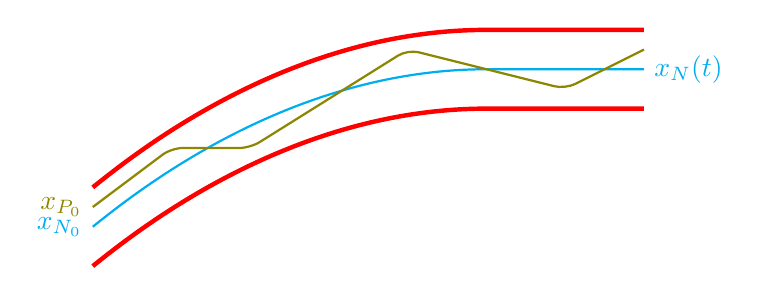
\begin{tikzpicture}
				\assistd{7}{t}{4}{x}
				\draw[ultra thick,color=red] (0,0) parabola[bend at end] (5,2)--(7,2);
				\draw[ultra thick,color=red] (0,1) parabola[bend at end] (5,3)--(7,3);
				\draw[color=cyan,thick] (0,.5)node[left]{$ x_{N_0} $} parabola[bend at end] (5,2.5)--(7,2.5) node[right]{$ x_N(t) $};
				\draw[color=olive,thick,rounded corners] (0,0.75)node[left]{$ x_{P_0} $} -- (1,1.5) -- (2,1.5)-- (4,2.75) -- (6,2.25) -- (7,2.75);
			\end{tikzpicture}
		\end{minipage}
	\end{figure}
	\lablsubsection{Asintotica stabilità del moto}
	Il moto $ x_N $(t) si dice \emph{Asintoticamente stabile} se  è stabile e:
	\begin{figure}[H]
		\begin{minipage}{0.5\textwidth}
			\begin{equation*}
				\Large\lim_{t\to+\infty}\vvline x_P(t) -x_N(t)\vvline=0
			\end{equation*}
			\[\forall x_{P_0}: \vvline x_P(t) -x_N(t)\vvline\leq\delta_\varepsilon\]
		\end{minipage}
		\begin{minipage}{0.5\textwidth}
			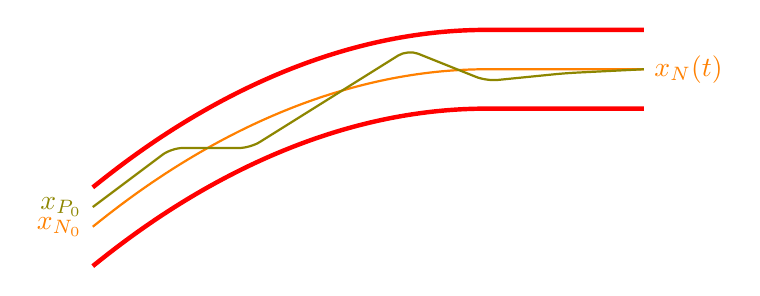
\begin{tikzpicture}
				\assistd{7}{t}{4}{x}
				\draw[ultra thick,color=red] (0,0) parabola[bend at end] (5,2)--(7,2);
				\draw[ultra thick,color=red] (0,1) parabola[bend at end] (5,3)--(7,3);
				\draw[color=orange,thick] (0,.5)node[left]{$ x_{N_0} $} parabola[bend at end] (5,2.5)--(7,2.5)node[right]{$ x_N(t) $};
				\draw[color=olive,thick,rounded corners] (0,0.75)node[left]{$ x_{P_0} $} -- (1,1.5) -- (2,1.5)-- (4,2.75) -- (5,2.35) -- (6,2.45) -- (7,2.5);
			\end{tikzpicture}
		\end{minipage}
	\end{figure}
	\lablsubsection{Instabilità del moto}
	\begin{figure}[H]
		\begin{minipage}{0.5\textwidth}
			Se non vale la condizione di stabilità, le traiettorie divergono e il moto si dice \emph{instabile}:
		\end{minipage}
		\begin{minipage}{0.5\textwidth}
			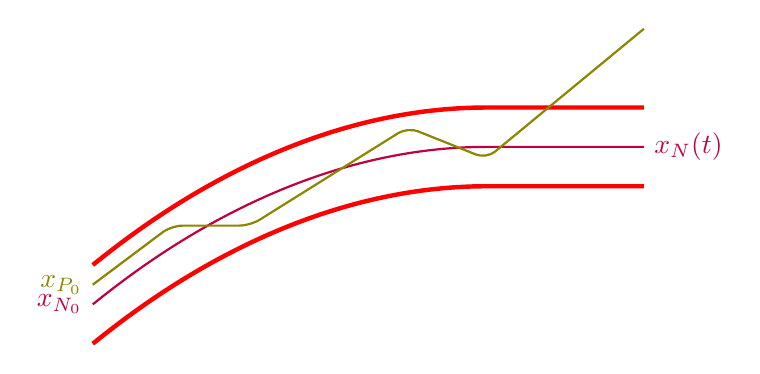
\begin{tikzpicture}
				\assistd{7}{t}{4}{x}
				\draw[ultra thick,color=red] (0,0) parabola[bend at end] (5,2)--(7,2);
				\draw[ultra thick,color=red] (0,1) parabola[bend at end] (5,3)--(7,3);
				\draw[color=purple,thick] (0,.5)node[left]{$ x_{N_0} $} parabola[bend at end] (5,2.5)--(7,2.5)node[right]{$ x_N(t) $};
				\draw[color=olive,thick,rounded corners] (0,0.75)node[left]{$ x_{P_0} $} -- (1,1.5) -- (2,1.5)-- (4,2.75) -- (5,2.35) -- (7,4);
			\end{tikzpicture}
		\end{minipage}
	\end{figure}
	Tutte le definizioni per ora scritte valgono anche per gli \emph{equilibri} (moti costanti), è sufficiente sostituire $ x_N(t) $ con $ \overline{x_N}\quad\forall t\geq0 $\\
	\nota{Gli equilibri possono soddisfare diverse definizioni di stabilità (vedi esempio seguente)}
	\begin{figure}[H]
		\centering
		\begin{minipage}{0.3\textwidth}
			\begin{tikzpicture}[font=\footnotesize]
				% Support
				\draw[pattern=dots] (0,0) circle(.25cm);
				\draw[->,color=purple] (0,-1) arc[start angle=-90,end angle=-60,radius=1];
				\draw[color=purple] (0.5,-0.75) node[right]{$ \tau = \vartheta $};
				\draw[color=darkgray] (0.25,0) node[above right]{Pendolo};
				\draw[dashed,color=gray] (0,0) -- (-90:4);
				% Rod + Bob
				\draw (0,0) -- (-60:4) node[fill,circle](m){};
				
				% Weight Force
				\draw[-latex] (m) -- node[right]{$\vec{Mg}$}++(0,-1) ;
			\end{tikzpicture}
			
		\end{minipage}
		\begin{minipage}{0.3\textwidth}
			\centering
			\begin{tikzpicture}[font=\footnotesize]
				% Support
				\draw[pattern=dots] (0,0) circle(.25cm);
				\draw[color=red] (-0.25,0) node[above left]{Instabile} node[below left,purple]{$ \tau = 180$° };
				\draw[->,color=purple] (0,-1) arc[start angle=-90,end angle =90,radius = 1];
				\draw[dashed,color=gray] (0,0) -- (-90:4);	
				% Rod + Bob
				\draw (0,0) -- (90:4) node[fill,circle](m){};
				
				% Weight Force
				\draw[-latex] (m) -- node[right]{$\vec{Mg}$}++(0,-1) ;
			\end{tikzpicture}
		\end{minipage}
		\begin{minipage}{0.3\textwidth}
			\centering
			\begin{tikzpicture}[font=\footnotesize]
				% Support
				\draw[pattern=dots] (0,0) circle(.25cm);
				\draw[color=green] (0.25,0) node[above right]{Stabile} node[below right]{$\tau =0$°};
				% Rod + Bob
				\draw (0,0) -- (-90:4) node[fill,circle](m){};
				
				% Weight Force
				\draw[-latex] (m) -- node[right]{$\vec{Mg}$}++(0,-1) ;
			\end{tikzpicture}
		\end{minipage}
	\end{figure}
	\lablsubsection{Regione di attrazione}
	Per gli stati \emph{Asintoticamente stabili} definiamo regione di attrazione l'insieme dei punti partendo dai quali si converge all'equilibrio.
	\begin{figure}[H]
		\centering
		\begin{tikzpicture}
			\newcommand{\var}{4}
			\assi{-\var}{\var}{x_1}{-\var}{\var-1}{x_2}
			\filldraw[color=darkpurple] (0,0) node[fill,circle](m){};
			\draw[color=darkpurple] (0,0) node[above right] {Equilibrio};
			\draw[color=red,rotate=45,thick] (2,1) -- (0,1) node[red,rotate=45,above,in front of path,scale=1.25] {Regione di attrazione} -- (-2,1) -- (-3,-2) -- (3,-2)--cycle;
		\end{tikzpicture}
	\end{figure}
	\nointerlineskip


%%% Local Variables:
%%% mode: latex
%%% TeX-master: "master"
%%% End:
